\documentclass[a4paper,11pt]{article}
\usepackage[margin=1in]{geometry}
\usepackage{amsmath,amsfonts,amssymb}
\usepackage{mathtools}
\usepackage{enumitem}
\usepackage{graphicx}
\usepackage{epstopdf} %converting to PDF
\usepackage{cancel}
\usepackage[font=small,labelfont=bf]{caption}
\renewcommand{\figurename}{Şekil}
\usepackage{multicol}
\usepackage{titling}
\usepackage{tikz}
\usetikzlibrary{shapes,arrows}
\renewcommand\maketitlehooka{\null\mbox{}\vfill}
\renewcommand\maketitlehookd{\vfill\null}
\usepackage[T1]{fontenc}
\usepackage[utf8]{inputenc}
\graphicspath{ {./images/} }
\title{KON313 - Geribeslemeli Kontrol Sistemleri \\ Ödev 1}
\date{}
\author{
    Mertcan Ekiz \\ 040160420
    \and
    Ömer Furkan Esen \\ 040150423
}
\begin{document}
\tikzstyle{block} = [draw, rectangle, 
    minimum height=3em, minimum width=5em]
\tikzstyle{sum} = [draw, circle, node distance=1cm]
\tikzstyle{input} = [coordinate]
\tikzstyle{output} = [coordinate]
\tikzstyle{pinstyle} = [pin edge={to-,thin,black}]
\maketitle
\newpage

\textbf{Soru 1:} Aşağıda bir kapalı çevrimli kontrol sisteminin blok şeması \mbox{verilmiştir.}

\begin{figure}[h]
    \centering
    \begin{tikzpicture}[auto, node distance=2cm,>=latex']
        % We start by placing the blocks
        \node [input, name=input] {};
        \node [sum, right of=input] (sum) {};
        \node [block, right of=sum, node distance=2.5cm] (controller) {$F(s)$};
        \node [block, right of=controller,
                node distance=3cm] (system) {$G(s)$};
        % We draw an edge between the controller and system block to 
        % calculate the coordinate u. We need it to place the measurement block. 
        \draw [->] (sum) -- node[below,name=e] {$E(s)$} (controller);
        \draw [->] (controller) -- node[name=u]{} (system);
        \node [sum, right of=system, node distance=2cm] (amplified) {};
        \node [block, above of=u, node distance=1.75cm] (k) {$K$};
        \node [output, right of=amplified] (output) {};
        \node [block, below of=u] (measurements) {$H(s)$};
    
        % Once the nodes are placed, connecting them is easy. 
        \draw [draw,->] (input) -- node {$R(s)$} (sum);
        % \draw [->] (sum) -- node[below] {$E(s)$} (controller);
        \draw [->] (system) -- (amplified);
        \draw [->] (amplified) -- node [name=y] {$Y(s)$}(output);
        \draw [->] (k) -| (amplified);
        \draw [draw, ->] (e) |- (k);
        \draw [->] (y) |- (measurements);
        \draw [->] (measurements) -| node[left,pos=0.96] {$-$} 
            node [near end] {} (sum);
    \end{tikzpicture}
    \caption{Kapalı çevrim kontrol sistemi}
    \label{fig:1}
\end{figure}

\begin{enumerate}[label=\textbf{\alph*}{.}, leftmargin=\parindent]
    \item Sistemin \emph{açık çevrim} ve \emph{kapalı çevrim} transfer fonksiyonlarını yazınız. \emph{İkinci mertebeden} olduğu bilinen $G(s)$ sistemine ilişkin birim basamak yanıtı Şekil 2'deki gibi olduğuna göre, $G(s)$ transfer fonksiyonunu bulunuz. Sistemin \emph{sönüm oranı} ($\zeta$) ve \emph{doğal frekansı} ($\omega_n$) nedir?
    \begin{figure}[h]
        \centering
        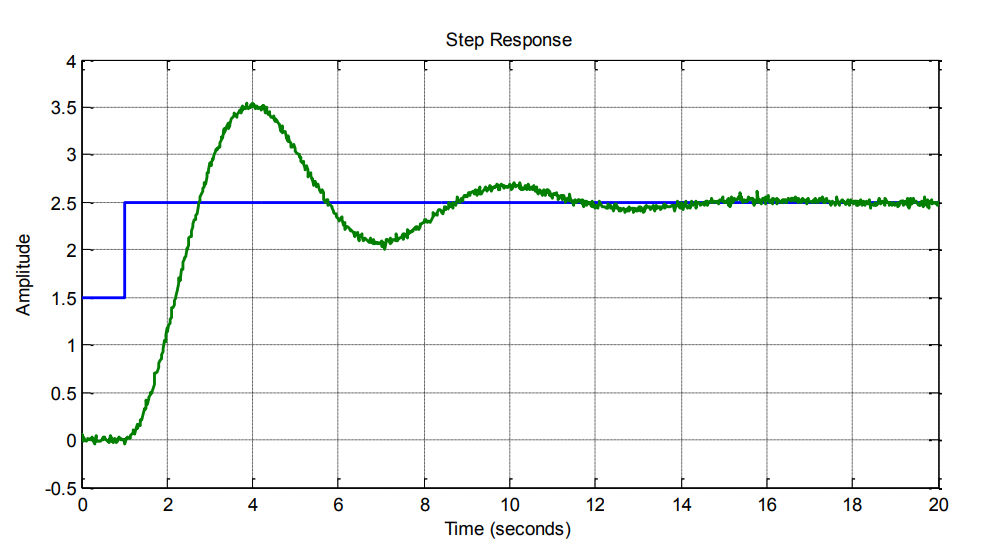
\includegraphics[width=0.9\textwidth]{fig1.png}
        \caption{İkinci mertebeden bir sistemin basamak yanıtı}
        \label{fig:2}
    \end{figure}
    \item $G(s)$ transfer fonksiyonu için, \emph{aşımı değiştirmeden} tepe zamanını yarıya indirmek isteniyor. Buna göre hangi parametre değiştirilmelidir ve bu parametrenin yeni değeri ne olmalıdır?
    \newpage
    \textbf{Çözüm:}
    Sistemin ileri yöndeki ($E(s) \rightarrow Y(s)$ arası) blok diyagramı sadeleştirilirse aşağıdaki eşdeğer sistem elde edilir:
    \begin{figure}[h]
        \centering
        \begin{tikzpicture}[auto, node distance=2cm,>=latex']
            % We start by placing the blocks
            \node [input, name=input] {};
            \node [sum, right of=input] (sum) {};
            \node [block, right of=sum, node distance=2.5cm] (controller) {$K + F(s)G(s)$};
            % We draw an edge between the controller and system block to 
            % calculate the coordinate u. We need it to place the measurement block. 
            \draw [->] (sum) -- node[below,name=e] {$E(s)$} (controller);
            \node [output, right of=controller,node distance=4cm] (output) {};
            \node [block, below of=controller] (measurements) {$H(s)$};
        
            % Once the nodes are placed, connecting them is easy. 
            \draw [draw,->] (input) -- node {$R(s)$} (sum);
            % \draw [->] (sum) -- node[below] {$E(s)$} (controller);
            % \draw [->] (controller) -- (amplified);
            \draw [->] (controller) -- node [name=y] {$Y(s)$}(output);
            \draw [->] (y) |- (measurements);
            \draw [->] (measurements) -| node[left,pos=0.8] {$B(s)$} 
                node [near end] {} (sum);
        \end{tikzpicture}
        \label{fig:simple1}
    \end{figure}

    Bu durumda açık çevrim transfer fonksiyonu $\frac{B(s)}{E(s)}$, kapalı çevrim transfer fonksiyonu ise $\frac{Y(s)}{R(s)}$ olur. Gerekli işlemler yapıldığında
    \begin{gather*} 
        \frac{B(s)}{E(s)} = (K + F(s)G(s))H(s)\,,\quad
        \frac{Y(s)}{R(s)} = \frac{K + F(s)G(s)}{1 + (K + F(s)G(s))H(s)}
    \end{gather*}

    olarak bulunur.\\[1em]
    İkinci mertebeden olduğu bilinen $G(s)$ sistemi, $\omega_n$ ve $\zeta$ cinsinden şu şekilde yazılabilir:
    \[ G(s) = \frac{K \omega_n^2}{s^2 + 2\zeta\omega_n s + w_n^2}\]
    Grafikten DC kazancın yaklaşık 2.5 olduğu görülmektedir ($K \approx 2.5$). Sönüm oranını bulmak için aşım miktarı incelebilir. Grafikte aşımın yaklaşık $\frac{3.5 - 2.5}{2.5} = 0.4$ olduğu görülmektedir. $ \text{Aşım} = OS = e^{-(\pi\zeta / \sqrt{1-\zeta^2})} $ olduğuna göre,
    \[ \zeta = \frac{-\ln{(OS)}}{\sqrt{\pi^2 + \ln^2{(OS)}}} = \frac{-\ln{(0.4)}}{\sqrt{\pi^2 + \ln^2{(0.4)}}} \approx 0.28\]
    olarak bulunur. Grafikten tepe zamanının yaklaşık 3 saniye olduğu görülmektedir. Bu değer aşağıdaki formüle koyulduğunda $\omega_n$ bulunabilir:
    \[ t_p = \frac{\pi}{\omega_n\sqrt{1-\zeta^2}} \quad\Rightarrow\quad 3 = \frac{\pi}{\omega_n\sqrt{1 - (0.28)^2}} \,,\; \omega_n \approx 1.09 \]
    Aşımı değiştirmeden tepe zamanını yarıya indirmek için paydada bulunan doğal frekansın iki katına çıkarılması gerekmektedir. Bu durumda yeni $\omega_n \approx 2.18$, yeni $t_p = 1.5$s olur. Birinci ve ikinci durumlardaki transfer fonksiyonları aşağıdaki gibidir.
\begin{gather*}
    G_1(s) = \frac{K\omega_n^2}{s^2 + 2\zeta\omega_n s + \omega_n^2} = \frac{2.975}{s^2 + 0.61s + 1.19} \approx \frac{3}{s^2 + 0.6s + 1.2} \\[0.8em]
    G_2(s) = \frac{K(4\,\omega_n^2)}{s^2 + 2\zeta(2\omega_n) s + 4\,\omega_n^2} = \frac{11.9}{s^2 + 1.22s + 4.76} \approx \frac{12}{s^2 + 1.2s + 4.8}
\end{gather*}
    \newpage\item $F(s) = \frac{0.1(s^2 - 0.2s + 1.25)}{s}$, $H(s) = 1$ ve $K = 0$ alındığı durumda kapalı çevrim sistemin kutup ve sıfırlarının yerlerini hesaplayın ve $s$-düzleminde gösterin. Sistem kararlılığını yorumlayın.\\[1em]
    \textbf{Çözüm:} İlk kısımda buldugumuz $G(s)$ sistemini de yerine koyduğumuzda sistemin kapalı çevrim transfer fonksiyonu aşağıdaki gibi olur:
    \begin{gather*}
        \frac{Y(s)}{R(s)} = \frac{F(s)G(s)}{1 + F(s)G(s)} = \frac{\frac{0.1(s^2 - 0.2s + 1.25)}{s} \times \frac{3}{s^2 + 0.6s + 1.2}}{1 + \frac{0.1(s^2 - 0.2s + 1.25)}{s} \times \frac{3}{s^2 + 0.6s + 1.2}}  \\[1em]
        = \frac{0.3 (s^2 - 0.2s + 1.25)}{s(s^2 + 0.6s + 1.2) + 0.3 (s^2 - 0.2s + 1.25)}
    \end{gather*}
    Bu durumda payın 2 kökü, paydanın 3 kökü, dolayısıyla da sistemin 2 sıfırı ve 3 kutbu olduğu görülmektedir. Bu kutuplar ve sıfırlar yaklaşık olarak aşağıdaki gibidir:

    \begin{gather*}
        \begin{split}
            p_1 \approx -0.4 \\
            p_2 \approx -0.25 - 0.94i\\
            p_2 \approx -0.25 + 0.94i
        \end{split}
        \quad\quad
        \begin{split}
            z_1 \approx 0.1 - 1.11i\\
            z_2 \approx 0.1 + 1.11i
        \end{split}    
    \end{gather*}
    \begin{figure}[h]
        \centering
        \begin{tikzpicture}[x=12cm,y=2cm]
            % Axes:
            \draw [-latex] (-.5,0) -- (.3,0) node [above left]  {Re};
            \draw [-latex] (0,-1.7) -- (0,1.7) node [below right] {Im};
            %ticks
        %     \foreach \x in {0,...,10}
        %     \draw (\x,1pt) -- (\x,-3pt)
        % node[anchor=north] {\x};
            \foreach \x in {-0.4, -0.3, -0.2, -0.1, 0.1, 0.2}
                \draw (\x,1pt) -- (\x,-3pt)
                    node[anchor=north] {\tiny{\x}};
            \foreach \y in {-1.5,-1.2,-0.9, -.6, -.3, .3, .6, .9, 1.2, 1.5}
                    \draw (1pt,\y) -- (-3pt,\y) 
                        node[anchor=east] {\tiny{\y}}; 

            \draw (-.4,0) node[above left] {$p_1$} node[solid, ultra thick, cross out,draw=red!80!black,inner sep=0pt,minimum size=5pt] {};
            \draw[dashed] (0,-.94) -- node[pos=0.99, below left] {$p_2$}(-.25,-.94) node[solid, ultra thick, cross out,draw=red!80!black,inner sep=0pt,minimum size=5pt] {} -- (-.25, 0);
            \draw[dashed] (0,.94) -- node[pos=0.99, above left] {$p_3$}(-.25,.94) node[solid, ultra thick, cross out,draw=red!80!black,inner sep=0pt,minimum size=5pt] {} -- (-.25, 0);
            % \draw[red, -stealth] (0,2) arc (90:145:2);
            
            % \draw[dashed] (0,0) -- node[pos=0.8, above right] {$\omega_z$}(125:3.5) node[solid, fill=white, circle,draw=black] {};
            % \draw[blue, -stealth] (0,1) arc (90:125:1);
            
            % \draw[dashed]  (-5,0) node[below left] {$-\zeta_p\omega_p$} --  (-5,-3) node[solid, cross out,draw=black] {};
            \draw[dashed]  (0,-1.11355) -- node[pos=0.99,below right]{$z_1$} (0.1,-1.11355) node[solid, fill=white, ultra thick, circle,draw=blue!80,inner sep=0pt,minimum size=7pt] {} -- (0.1, 0);
            \draw[dashed]  (0,1.11355) -- node[pos=0.9,above right]{$z_2$} (0.1,1.11355) node[solid, fill=white, ultra thick, circle,draw=blue!80,inner sep=0pt,minimum size=7pt] {} -- (0.1, 0);
        \end{tikzpicture}
    \end{figure}

    Sistemin kutuplarından hiçbiri imajiner eksenin sağ tarafında olmadığı için sistem kararlıdır.
    \newpage\item $F(s) = H(s) = 1$ olduğu durumda kapalı çevrim sistem kutuplarının $s_{1,2} = -0.3 \pm 1.9i$ noktalarında konumlanması için $K$ ne seçilmelidir? Bu $K$ değeri ile birlikte $E(s)$ ifadesini elde ediniz. $R(s) = \frac{1}{s}$ olarak verildiği durumda $\lim\limits_{t\rightarrow\infty} e(t)$ ifadesinin değerini hesaplayınız.\\[1em]
    \textbf{Çözüm:} $F(s) = H(s) = 1$ olduğu durumda sistemin kapalı çevrim transfer fonksiyonu aşağıdaki gibidir:
    \begin{gather*}
        \frac{Y(s)}{R(s)} = \frac{ K + G(s) }{1 + K + G(s)} = 1 - \frac{ 1 }{1 + K + G(s)}\\[0.8em]
        = 1 - \frac{s^2 + 0.6s + 1.2}{(1+K)(s^2 + 0.6s + 1.2) + 3}
    \end{gather*}
    Kutupları bulmak için payda sıfıra eşitlenir ve verilen $s$ değerleri yerine koyulur:
    \begin{gather*} 
        (1+K)(s^2 + 0.6s + 1.2) + 3 = 0
    \end{gather*}
    Burada $s_{1,2}$'den herhangi biri yerine koyulursa $K = 0.2$ olarak bulunur.\\[1em]
    $E(s)$ ifadesini $R(s)$ cinsinden elde etmek için sistemin kapalı çevrim transfer fonksiyonu kullanılabilir.
    \begin{gather*}
        \frac{Y(s)}{R(s)} = 1 - \frac{ 1 }{1 + K + G(s)}\\[.8em]
        E(s) = R(s) - Y(s) = R(s)\left[1 - \left(1 - \frac{ 1 }{1 + K + G(s)}\right)\right] \\[0.8em]
        E(s) = R(s)\left(\frac{1}{1 + K + G(s)}\right) \\[0.8em]
    \end{gather*}
    $R(s)$, $G(s)$ ve $K$ değerleri yerine koyulursa ve son değer teoremi uygulanırsa:
    \begin{gather*}
        \lim\limits_{t\to\infty}e(t) = \lim\limits_{s\to 0} \;sE(s) = \lim\limits_{s\to 0} \; s \,\frac{1}{s}\,\frac{1}{\left(1.2 + \frac{3}{s^2 + 0.6s + 1.2}\right)} = \frac{1}{1.2 + \frac{3}{1.2}} \approx 0.27
    \end{gather*}
\end{enumerate}

\newpage\textbf{Soru 2:} Aşağıda verilen mekanik sistem için soruları cevaplandırınız.
\begin{figure}[h]
    \centering
    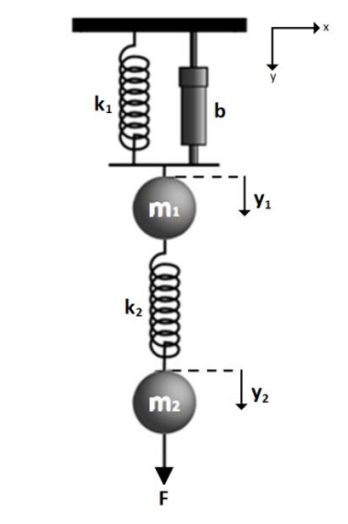
\includegraphics[height=5cm]{fig2.png}
    \caption{İki serbestlik dereceli mekanik sistem}
    \label{fig:3}
\end{figure}
\begin{enumerate}[label=\textbf{\alph*}{.}]
\item X ekseninde herhangi bir hareketin olmadığını varsayarak, sisteme ilişkin hareket denklemlerini yazınız. Sistemin \emph{durum uzayı modelini}, durum değişkenlerini
\begin{gather*}
    x_1 = y_1 \,,\quad x_3 = y_2\\
    x_2 = \dot{y}_1 \,,\quad x_4 = \dot{y}_2
\end{gather*}
alarak elde ediniz.
\item Sisteme ilişkin $G(s) = \frac{Y_1(s)}{F(s)}$ transfer fonksiyonunun

\begin{gather*}
    G(s) = \frac{25}{s^4 + 4s^3 + 125s^2 + 100s + 625}
\end{gather*}

olduğunu gösteriniz. (Laplace dönüşümü sırasında yerçekimini bozucu etki olarak düşünüp ihmal edebilirsiniz.) Sistemin \emph{kutuplarını} hesaplayınız ve $s$-tanım bölgesinde gösteriniz. Sistemin \emph{mertebesi} nedir?\\[1em]
\textbf{Çözüm:} $m_1$ ve $m_2$ kütleleri üzerine etki eden kuvvetleri ayrı ayrı yazarsak:\\[1em]
\begin{equation}
    \begin{gathered}
        m_1\ddot{y}_1 + b\dot{y}_1 + (k_1 + k_2)y_1 = k_2 y_2\\
        \ddot{y}_1 = \frac{-b}{m_1}\dot{y}_1 - \frac{k_1 + k_2}{m_1}y_1 + \frac{k_2}{m_1}y_2
    \end{gathered}
\end{equation}\\
\begin{equation}
    \begin{gathered}
        m_2\ddot{y}_2 + k_2 y_2 = k_2 y_1 + F\\
        \ddot{y}_2 = \frac{k_2}{m_2}y_1 - \frac{k_2}{m_2}y_2 + \frac{F}{m_2}
    \end{gathered}
\end{equation}\newpage
\begin{gather*}
    \begin{split}
        \dot{\mathbf{x}} = \mathrm{A}\mathbf{x} + \mathrm{B}\,u(t)\\
        \mathbf{y} = \mathrm{C}\mathbf{x} + \mathrm{D}\,u(t)
    \end{split}
    \quad\quad\quad\quad
    \begin{split}
        \mathbf{x} = \begin{bmatrix}
            y_1 \\
            \dot{y}_1\\
            y_2 \\
            \dot{y}_2
        \end{bmatrix}
    \end{split}
    \quad\quad
    \begin{split}
        u(t) = F
    \end{split}
\end{gather*}
(1) ve (2) numaralı eşitlikler, yukarıdaki durum uzayı matrislerine uygun bir şekilde yerleştirilip Tablo 1'deki değerler yerine koyulursa sistemin durum uzayı modeli elde edilir.
\begin{gather*}
    \begin{bmatrix}
        \dot{y}_1 \\
        \ddot{y}_1 \\
        \dot{y}_2 \\
        \ddot{y}_2
    \end{bmatrix}
    =
    \begin{bmatrix}
        0 & 1 & 0 & 0 \\
        -100 & -4 & 75 & 0 \\
        0 & 0 & 0 & 1 \\
        25 & 0 & -25 & 0
    \end{bmatrix}
    \begin{bmatrix}
        y_1 \\ \dot{y}_1 \\ y_2 \\ \dot{y}_2
    \end{bmatrix}
    +
    \begin{bmatrix}
        0 \\ 0 \\ 0 \\ \frac{1}{3}
    \end{bmatrix}
    u(t) \\[1em]
    \mathbf{y} = \begin{bmatrix}
        1 & 0 & 0 & 0
    \end{bmatrix}
    \begin{bmatrix}
        y_1 \\ \dot{y}_1 \\ y_2 \\ \dot{y}_2
    \end{bmatrix}
\end{gather*}
Transfer fonksiyonunu elde etmek içinse (1) ve (2) numaralı eşitliklerin Laplace dönüşümleri alınır:
\begin{gather*}
    m_1 s^2 Y_1(s) + b s Y_1(s) + (k_1 + k_2) Y_1(s) = k_2 Y_2(s) \\
    m_2 s^2 Y_2(s) + k_2 Y_2(s) = k_2 Y_1(s) + F(s)
\end{gather*}
Denklemler sadeleştirilerek $F(s)$, $Y_1(s)$ cinsinden yazılır ve Tablo 1'deki değerler yerine konursa:
\begin{gather*}
    Y_1(s)\left(\frac{m_1 s^2 + b s + k_1 + k_2}{k_2} \times (m_2 s^2 + k_2) - k_2\right) = F(s)\\
    Y_1(s)\left(\frac{s^2 + 4s + 100}{75} \times (3s^2 + 75) - 75\right) = F(s)\\
    Y_1(s)\left(\frac{s^4 + 4s^3 + 125s^2 + 100s + 625}{25}\right) = F(s)  \\[0.8em]
    G(s) = \frac{Y_1(s)}{F(s)} = \frac{25}{s^4 + 4s^3 + 125s^2 + 100s + 625}
\end{gather*}
olarak bulunur.

\newpage Transfer fonksiyonunun paydasının derecesi 4 olduğuna göre sistemin mertebesi de 4'tür. Dolayısıyla sistemin 4 adet kutbu vardır. Bu kutuplar yaklaşık olarak aşağıdaki gibidir:

\begin{figure}[h]
    \centering
    \begin{tikzpicture}[x=1.7cm,y=.3cm]
        % Axes:
        \draw [-latex] (-2,0) -- (2,0) node [above left]  {Re(s)};
        \draw [-latex] (0,-12) -- (0,12) node [below right] {Im(s)};
        %ticks
        \foreach \x in {-1.5, -1.0, -0.5, 0, 0.5, 1.0, 1.5}
            \draw (\x,1pt) -- (\x,-3pt)
                node[anchor=north] {\tiny{\x}};
        \foreach \y in {-10,-8,-6,-4,-2,2,4,6,8,10}
                \draw (0pt,\y) -- (-3pt,\y) 
                    node[anchor=west, node distance=10pt] {\tiny{\y}}; 

        \draw[dashed] (0,-10.70) -- node[pos=0.99, below left] {$p_1$}(-1.65,-10.70) node[solid, ultra thick, cross out,draw=red!80!black,inner sep=0pt,minimum size=5pt] {} -- (-1.65, 0);
        \draw[dashed] (0,10.70) -- node[pos=0.99, above left] {$p_2$}(-1.65,10.70) node[solid, ultra thick, cross out,draw=red!80!black,inner sep=0pt,minimum size=5pt] {} -- (-1.65, 0);

        \draw[dashed] (0,-2.28) -- node[pos=0.99, below left] {$p_3$}(-0.35,-2.28) node[solid, ultra thick, cross out,draw=red!80!black,inner sep=0pt,minimum size=5pt] {} -- (-0.35, 0);
        \draw[dashed] (0,2.28) -- node[pos=0.99, above left] {$p_4$}(-0.35,2.28) node[solid, ultra thick, cross out,draw=red!80!black,inner sep=0pt,minimum size=5pt] {} -- (-0.35, 0);
    \end{tikzpicture}
    \begin{gather*}
        p_{1,2} \approx -1.65 \pm 10.70i \\
        p_{3,4} \approx -0.35 \pm 2.28i
    \end{gather*}
    \caption{Sistemin kutupları}
    \label{fig:poles}
\end{figure}
\item Sistem $F(s) = 15$ olarak verilen P tipi bir kontrolör ile kapalı çevrime alınsın (Şekil 5). Bu durumda kapalı çevrim sistemin yaklaşık yerleşme süresini, sönüm oranını ve aşım miktarını hesaplayınız (Yüksek mertebeden sistemlerde sistem davranışı üzerinde baskın kutupların etkisinin en fazla olduğunu unutmayın).
\begin{figure}[h]
    \centering
        \begin{tikzpicture}[auto, node distance=2cm,>=latex']
            % We start by placing the blocks
            \node [input, name=input] {};
            \node [sum, right of=input] (sum) {};
            \node [block, right of=sum] (controller) {$F(s)$};
            \node [block, right of=controller, node distance=3cm] (system) {$G(s)$};
            % \node 
            % We draw an edge between the controller and system block to 
            % calculate the coordinate u. We need it to place the measurement block. 
            \draw [->] (controller) -- node[below,name=u] {} (system);
            \node [output, right of=system,node distance=3cm] (output) {};
            \coordinate [below of=u] (measurements);
        
            % Once the nodes are placed, connecting them is easy. 
            \draw [draw,->] (input) -- node {$R(s)$} (sum);
            \draw [->] (sum) -- (controller);
            % \draw [->] (controller) -- (amplified);
            \draw [->] (system) -- node [name=y] {$Y(s)$}(output);
            \draw (y) |- (measurements);
            \draw [->] (measurements) -| node[left,pos=0.9] {$-$} (sum);
        \end{tikzpicture}
    \caption{Birim geribeslemeli kapalı çevrim kontrol sistemi}
    \label{fig:4}
\end{figure}
\end{enumerate}
\textbf{Çözüm:} Bu durumda sistemin kapalı çevrim transfer fonksiyonu aşağıdaki gibi olur:
\begin{gather*}
    \frac{Y(s)}{R(s)} = \frac{F(s)G(s)}{1 + F(s)G(s)} = \frac{15 \times \frac{25}{s^4 + 4s^3 + 125s^2 + 100s + 625}}{1 + 15 \times \frac{25}{s^4 + 4s^3 + 125s^2 + 100s + 625}} \\[.8em]
    = \frac{375}{s^4 + 4s^3 + 125 s^2 + 100s  + 1000}
\end{gather*}
4. dereceden olan bu sistemin 4 tane kutbu vardır ve yaklaşık değerleri aşağıdaki gibidir:
\begin{gather*}
    p_{1,2} = -1.69 \pm 10.55i\\
    p_{3,4} = -0.31 \pm 2.94i
\end{gather*}
Bu kutuplardan orijine daha yakın olanları ($p_3$ ve $p_4$) baskın kutup olacağından ve sistemin davranışını belirleyeceğinden dolayı, sistem sanki sadece bu iki kutuptan oluşan bir ikinci mertebeden sistemmiş gibi davranıp, yaklaşık sistem karakteristiklerine ulaşılabilir.

\begin{gather*}
    \frac{Y(s)}{R(s)} \approx \frac{K}{(s-p_3)(s-p_4)} = \frac{K}{(s+0.31-2.94i)(s+0.31+2.94i)} = \frac{\omega_n^2}{s^2 + 2\zeta\omega_n s + \omega_n^2}\\[.8em]
    (s + 0.31 - 2.94i)(s + 0.31 + 2.94i) = s^2 + 0.62s + 8.74 = s^2 + 2\zeta\omega_n s + \omega_n^2\\
    8.74 = \omega_n^2 \;\Rightarrow\; \omega_n \approx 2.96 \;,\qquad 2\zeta\omega_n = 0.62 \;\Rightarrow\; \zeta \approx 0.1 \\[1.2em]
    t_s = \frac{4}{\zeta\omega_n} \approx 12.88\mathrm{s} \qquad \text{(\%2'lik bant için)}\\
    t_s = \frac{3}{\zeta\omega_n} \approx 9.66\mathrm{s} \qquad \text{(\%5'lik bant için)}\\[1.2em]
    \text{\%Aşım} = 100 \times e^{(-\pi\zeta / \sqrt{1-\zeta^2})} \approx \%72
\end{gather*}
\newpage\textbf{Soru 3:} Aşağıda verilen sistemlerin birim basamak yanıtlarını MATLAB ile çizdiriniz ve bu yanıtlar arasındaki farkların nedenlerini yorumlayınız

\begin{enumerate}[label=\alph*)]
\item $\displaystyle\frac{7s + 20}{2s^2 + 5s + 20}$

\begin{figure}[h]
    \centering
    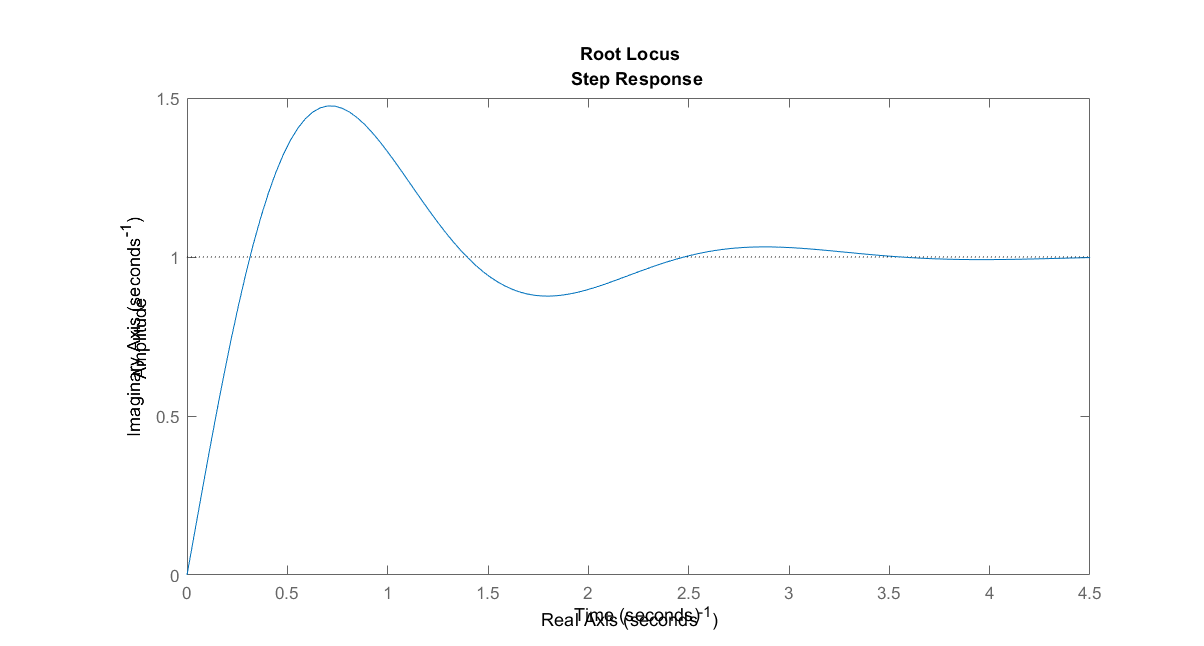
\includegraphics[width=.8\textwidth]{s1.png}
\end{figure}
Sistem az sönümlüdür. Beklenildiği gibi sonuç vermiştir.
\item $\displaystyle\frac{-7s+20}{2s^2 + 5s + 20}$

\begin{figure}[h]
    \centering
    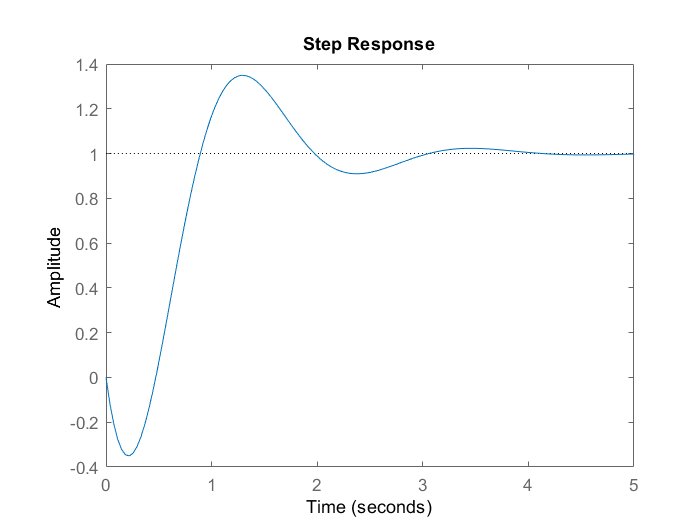
\includegraphics[width=.8\textwidth]{s2.png}
\end{figure}
Sistemin başlar başlamaz negatif yönde ilerlemesi G(s) nin pay kısmındaki -7s yüzündendir. Sisteme giren birim basamak fonksiyonuyla (1/s) beraber bu değer, sadece -7 değeriyle kalır ve bu da sistemi ilk halide negatif yönde ilerletir.
\newpage\item $\displaystyle\frac{20}{2s^2 + 5s + 20}$

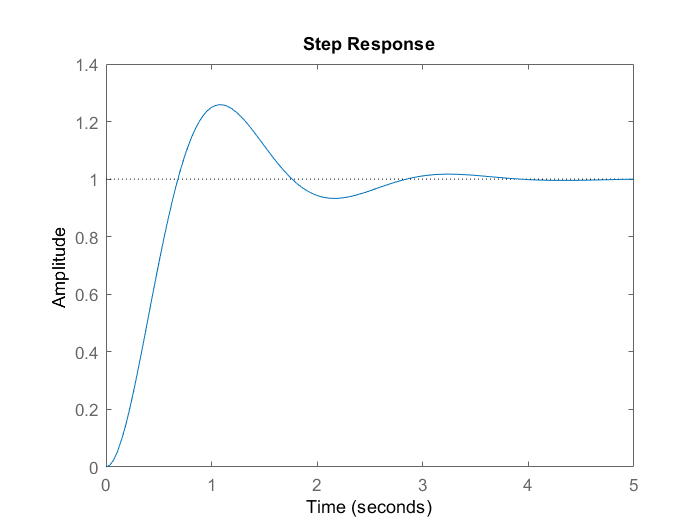
\includegraphics[width=.8\textwidth]{s3.png}
Sistemin grafiği a şıkkındakine çok benzer fakat küçük bir farkları vardır. bu da sıfır anından çıkış halinde c grafiği daha yatay bir halde çıkarken a grafiği birim basamak fonksiyonuyla çarpılan ve sonucunda +7 sayısını veren 7s'le beraber daha dik ve kesin bir yükselme sağlar. 
\item $\displaystyle\frac{7s}{2s^2 + 5s + 20}$

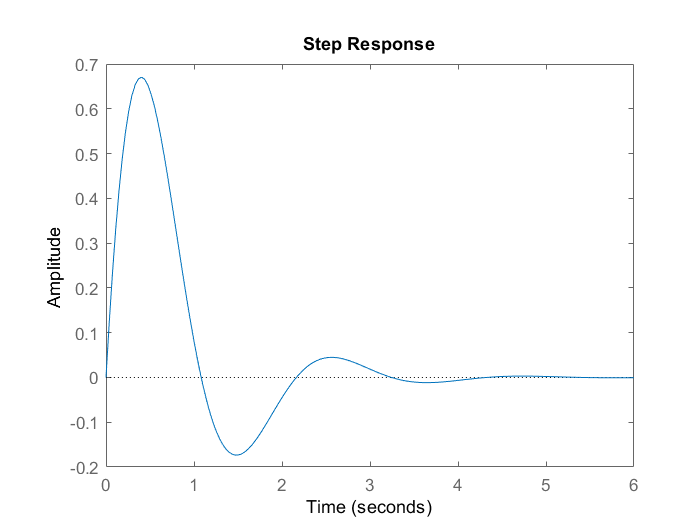
\includegraphics[width=.8\textwidth, height=.34\textheight]{s4.png}
Sistemin bu hali almasındaki temel neden basamak fonksyonunun da sisteme girmesiyle beraber pay kısmında sadece 7 ifadesinin kalmasına rağmen paydada 2. Dereceden bir denklem vardır. İlk pozitif yöndeki sıçramayı 7s sayısının pozitif olmasına bağlayabiliriz. Sıçramadan sonra 0 konumuna geri döner ve bir zaman sonra stabil kalır.
\newpage\item $\displaystyle\frac{-7s}{2s^2 + 5s + 20}$

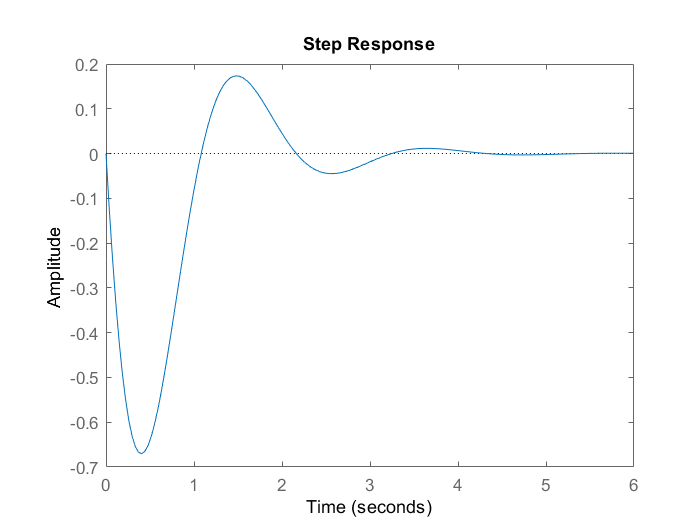
\includegraphics[width=.8\textwidth]{s5.png}
D'de verilen grafiğin aynısı sadece ilk başta pozitif yönde ilerlemek yerine negatif yönde ilerlemiş bu -7s'in önündeki eksi yüzünden olmuştur daha sonra eski sıfır haline döner.
\item $\displaystyle\frac{-20}{2s^2 + 5s + 20}$

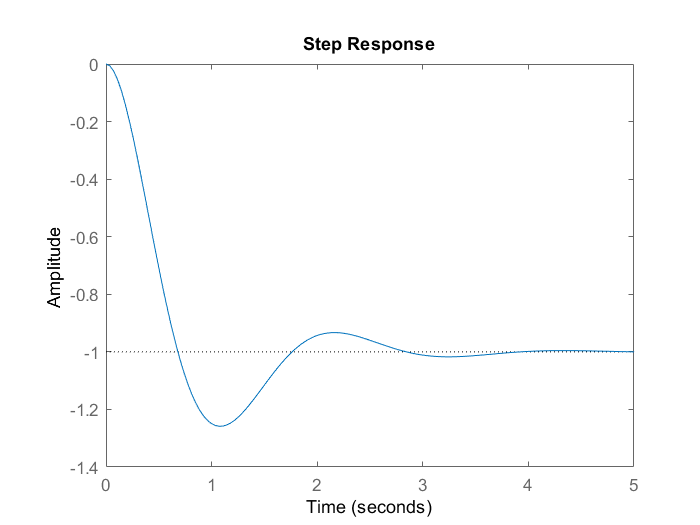
\includegraphics[width=.8\textwidth]{s6.png}
Yanında 7s veya -7s terimi olmayan sabit sayı birim basamak fonksyonunun girmesiyle beraber yine sistemi 1 e götürmüştür fakat paydanın önündeki negatif katsayı nedeniyle sistemi -1 e götürüp orada sabitlemiştir.
\end{enumerate}
\mbox{}\\

\textbf{Soru 4:}
\begin{figure}[h]
    \centering
    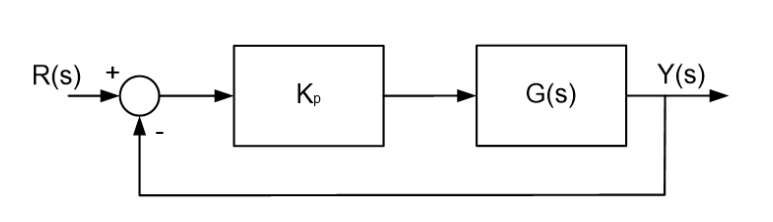
\includegraphics[width=0.75\textwidth]{fig4.png}
    \caption{Kapalı çevrim kontrol sistemi}
    \label{fig:5}
\end{figure}
Yukarıdaki blok diyagramındaki sistemin modeli \[ G(s) = \frac{s^3 + 18s^2 + 95s + 150}{s^3 + 3s^2 - 28s} \] biçimindedir. Buna göre,
\begin{enumerate}[label=\textbf{\alph*}{.}]
\item Pozitif $K_p$ değerleri için kapalı çevrimli sistemin köklerin değişimini gösteren grafiği çiziniz (Not: Kök eğrisini derste gösterilen adımları teker teker uygulayarak çizmeniz beklenmektedir).

\textbf{Çözüm:}
\begin{enumerate}[resume,label=\arabic*)]
    \item Kutup sayısı "3" $\longrightarrow (0, -7, 4)$ kutuplar \\
    Sıfır sayısı "3" $\longrightarrow (-3, -5, -10)$ sıfırlar
    \item Asimptot sayısı \\
    Kutup sayısı - Sıfır sayısı - $3 - 3 = 0$
    \item $\frac{DK}{DP}$ bulunması
    \begin{gather*}
        \frac{(s^3 + 18s^2 + 95s + 150)K_p}{s^3 + 3s^2 - 28s} + 1 = 0 \\[.8em]
        \frac{-(s^3 + 3s^2 - 28s)}{s^3 + 18s^2 + 95s + 150} = K_p \\[.8em]
        \frac{\sigma^3 + 3\sigma^2 - 28\sigma}{\sigma^3 + 18\sigma^2 + 95\sigma + 150} = K_p \\[.8em]
        \frac{\mathrm{d}\,K_p}{\mathrm{d}\sigma} \Rightarrow (3\sigma^2 + 6\sigma - 28)(\sigma^3 + 18\sigma^2 + 95\sigma + 150) = A \\[.8em]
        (3\sigma^2 + 36\sigma + 95)(\sigma^3 + 3\sigma^2 - 28\sigma) = B \\[1em]
        \frac{\mathrm{d}\,K_p}{\mathrm{d}\sigma} = \frac{A - B}{(\sigma^3 + 18\sigma^2 + 95\sigma + 150)^2} = 0 \\
        -8,5 \quad / \quad -4, 6 \quad / \quad 1.04 + 0.6i \quad / \quad 1.04 - 0.6i
    \end{gather*}
\end{enumerate}
\begin{enumerate}[resume*, start=6]
    \item İmajiner ekseni kesen kısımlar
    \begin{gather*}
        s^3(K_p + 1) + s^2(18K_p + 3) + s(95K_p - 28) + 150K_p \\[1em]
        \begin{array}{lcccc}
            s^3 & \| & K_p + 1 & 95K_p - 28 & 0 \\
            s^2 & \| & 18K_p + 3 & 150K_p & 0 \\
            s^1 & \| & \beta_1 & 0 & \\
            s^0 & \| & 150K_p & &
        \end{array}\\[1em]
        \frac{(95K_p - 28)(18K_p+3) - (K_p + 1)(150K_p)}{18K_p + 3} = \beta_1 \\[.8em]
        K_p > 0.39 \qquad \cancel{K_p > -1} \quad \cancel{K_p > -0.18} \quad \text{($K_p$ sıfırdan büyük)}\\
        K_p > 0.39 \;\Longrightarrow\; 10.11s^2 = -59 \\
        s = \pm 2.24j
    \end{gather*}
    \begin{figure}[h]
        \centering
        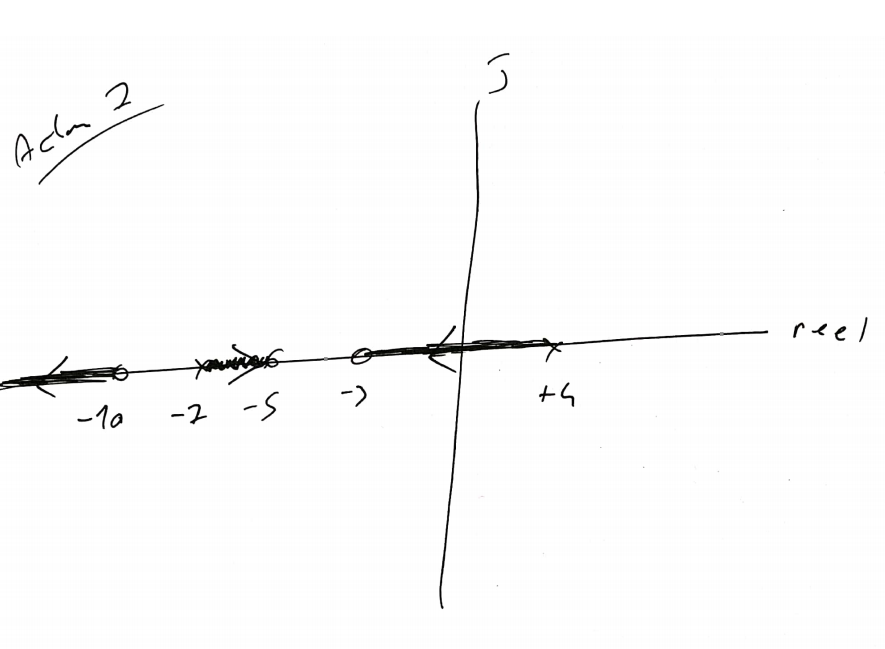
\includegraphics[width=1\textwidth]{step7.png}
    \end{figure}
\end{enumerate}
\newpage\item Grafiğin doğruluğunu test etmek için MATLAB'ta \texttt{ rlocus() } komutunu kullanarak kök eğrisini çizdiriniz.
\begin{figure}[h]
    \centering
    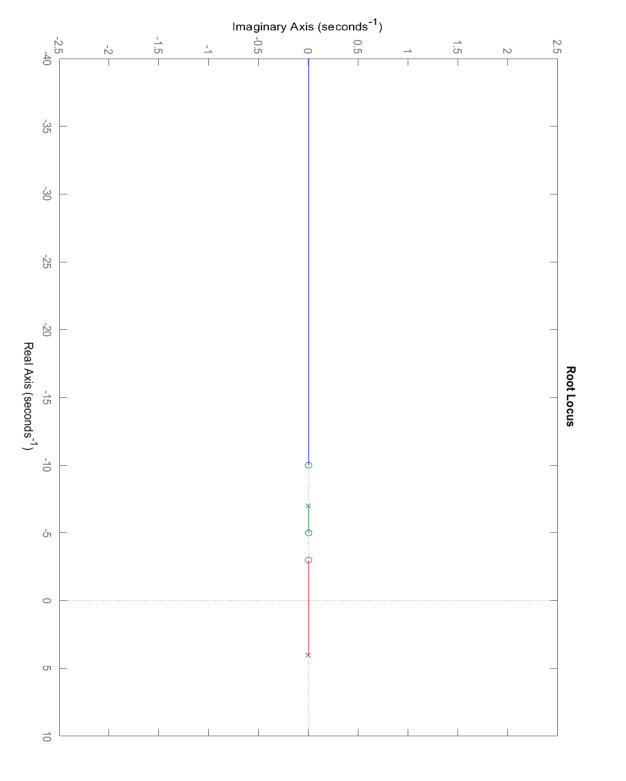
\includegraphics[width=.9\textwidth
    ]{rlocuss.png}
    \caption{MATLAB rlocus grafiği}
    \label{}
\end{figure}
\end{enumerate}
\end{document}